\chapter{Debugging, Testing and Results Evaluation}
\label{testing}



In order to ensure that the functionalities of the application have been achieved and abnormal/erroneous interactions have been eliminated, it is very important to debug and test a system as a whole and its individual parts during and thereafter the implementation. 
Over the development of the project, fro testing the correctness, completeness and quality of the application, the test process was divided into three main phases: unit testing\cite{unit}, responsiveness tests and system testing. Unit testing was performed throughout the development of the application while responsiveness testing and system testing were performed towards the completion of the development stage. In this chapter, the outcomes of all testing procedures will be discussed.


\section{Unit Testing with MSTest}
\label{unit_testing}

Unit tests are used to check and verify the smallest  possible part and component of the application. This component usually is the smallest testable part of the application and it usually has one or a few inputs and a single output. They allow programmers to examine the viability of the code as it is being developed. For example, a test could assert the outcome of an object's instance variables after it has been initialised, or after some other methods have been executed.


%elizabeth p.49
As mentioned, unit testing, was performed during the implementation of each of the components of the application and as additional functionalities were added, their individual performance was examined with small unit tests. The specific functionality that was just added, was then tested again, after it has been integrated with the rest of the application , in order to make sure that they functioned properly and didn't obstruct the functionality of any other component.

%Katherine Hinke
Microsoft and ASP.NET Core recognizes the big usefulness and importance of unit testing and thus Visual Studio Community 2017 ships with its own unit testing framework, known as MSTest or officially ``Visual Studio Unit Testing Framework'' which was used for this project. It comes with its own test suit, which proves a professional test guide to help developers write test code for unit testing.
In order to facilitate the unit testing of the application, three seperate classes were created:
\begin{enumerate}
\item \textbf{HomeControllerTests.cs}: This class test the functionality of the HomeController, which is the single controller of the application that handles the http requests coming from the browser. The proper functionality of this class was certainly of paramount importance, since the home controller is responsible for instantiating and manipulating the appropriate models and view models.  This class has in total five methods and thus the testing class has as well an equal amount of methods. It was very essential for the application that both the HttpGet and HttpPost methods were rigorously tested since their functionality is substantially different.
\item \textbf{DBContextTests.cs}: In this class the proper functionality of the database was tested in order to ensure security and the quality of the database. Since the home controller passes object to the DBContext for manipulation the accurate loading of the object had to be precisely ensured. The DBContext has in total 14 submethods and therefore the testing class has an equal amount of test methods.
\item \textbf{MediaUtilitiesTests.cs}: This class was created to help the application extract the metadata from the input files and therefore its absolute proper functionality was of high importance. It must have been ensured that this class could provide the right metadata of the media files, at any cases and under all extreme conditions. The bulk of the tests was done on this specific test class. 
 
\end{enumerate}

Following the pattern of true test-driven development (TDD)\cite{tdd1}\cite{tdd2},  a developer should follow three rules\cite{clean_coder} :

\begin{enumerate}
\item ``You are not allowed to write any production code until you have first written a failing unit test''
\item ``You are not allowed to write more of a unit test than is sufficient to fail-and not compiling is failing''
\item ``You are not allowed to write more production code that is sufficient to pass the currently failing unit test.''

\end{enumerate}


Being in line with the aforementioned approach,every time a single test was developed, the testing collection was run to ensure that all the previously created tests were successful and that the newly created test was failing. So, essentially, the tests for each method was created first and then the method in question was implemented. Once the newly implemented method was written, the collection of tests was run again in order to ensure not only that the specific test passed, but that no other test in the test suite was affected by the newly added method. At the end of the development stage, the tests suite was executed one more time in order to make sure that all written tests successfully passed, which they did. In the figure \ref{unit_tests} the result of each individual test is shown upon the completion of the test suite.


\begin{figure}[!ht]
\begin{center}
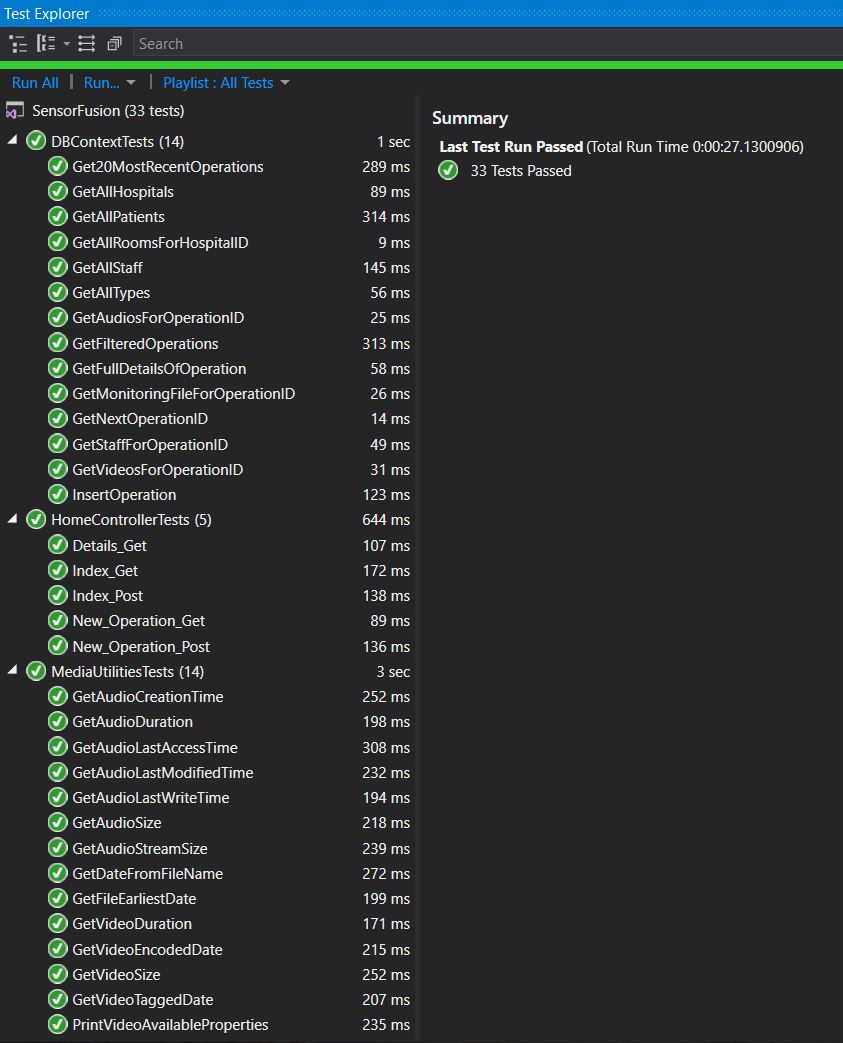
\includegraphics[width=17cm]{imgs/unit_tests.jpg}
\end{center}\vspace{-0.3cm}
\caption[Unit Test Report]{Summarised result from executing the entire test suite for the whole project} \label{unit_tests}
\end{figure}



\section{Responsiveness Tests-Cross Browser Compatibility}
\label{responsiveness_tests}

The application aims to be accessible to all doctors/users and all the NHS computers regardless of the browser installed on each computer. Therefore, the system must be responsive on a variety of client browsers. The application was tested for responsiveness on 5 browsers including Google Chrome, Mozilla Firefox, Opera, Internet Explorer and Microsoft Edge.

All pages of the application were tested in this session, one example can be seen in Figure \ref{responsiveness_test} which shows how one of the pages (the home page) tested performed on all of the aforementioned browsers. Part of the responsiveness test was also the display functionality such as the 	``chosen'' dropdown menus, multi-select dropdown menus, date-pickers etc. The responsive Bootstrap/CSS styled display was evaluated with acceptable performance on all browsers and only slight visual changes were made during this testing session so that a better user view for all users was possible.


\begin{figure}[!ht]
\begin{center}
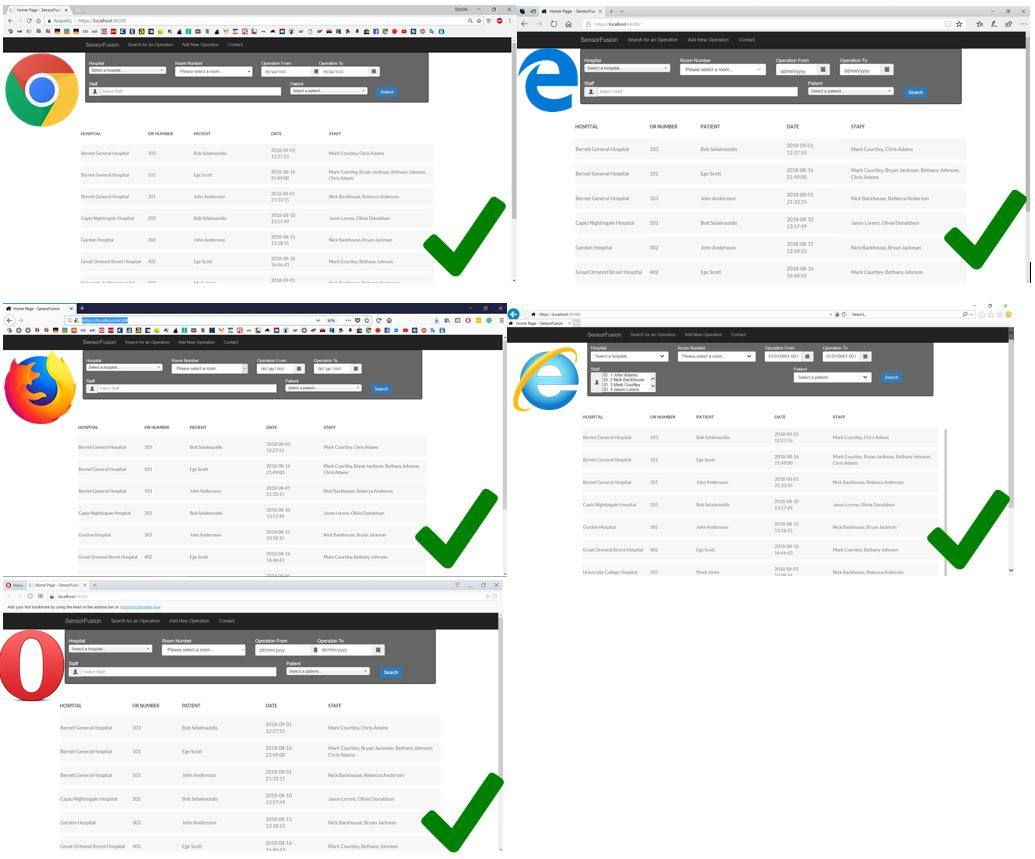
\includegraphics[width=17cm]{imgs/responsiveness_test.jpg}
\end{center}\vspace{-0.3cm}
\caption[Responsiveness Tests]{Screen shot of how the home page of the application is displayed on different browsers} \label{responsiveness_test}
\end{figure}


%look huajiang wang, lucas valti and 
\section{System Testing}
\label{system_testing}


The aim of system testing is to establish that the system meets the functional and non functional requirements defined in Chapter \ref{chapterlabel3} \cite{system_testing}. In the test plan that was followed, the test object in system testing was the whole application. At this phase, the testing method was to invite three volunteers to participate in the  test and ask them to finish a sequence of operations according to different scenarios. 




\begin{itemize}
  \item \textbf{Scenario one:}\\
  The volunteers are initially provided with sample operation's informations and files and are asked to upload the operation to the system. The volunteers can operate in their own way without any constrains or interference. 
    \item \textbf{Scenario two:}\\ 
The volunteers are asked to navigate to the home page and start searching for a specific operation using the pre-defined filters. The volunteers are then provided with all the information related to a specific operation and are asked to use the filters in order to find the stored operation in the database. The volunteers are then asked to load all the relevant information of the operation and view the details of the operation in question.
\end{itemize}


